\documentclass{article}
\usepackage{fancyhdr}
\usepackage{graphicx}
\usepackage{bbold}
\pagestyle{fancy}

\author{Philipp Kiss}

\lhead{Philipp Kiss}
\rhead{Grundlagen der Elektro- und Digitaltechnik}

\begin{document}
\pagenumbering{gobble}

\section{Einheiten}
\begin{table}[h!]
		\begin{center}
				\caption{Stromeinheiten}
				\label{tab:Stromeinheiten}
				\begin{tabular}{|c|c|p{7cm}|}
						\hline
						\textbf{Wert} & \textbf{Einheit} & \textbf{Beschreibung} \\
						\hline
						Spannung U & Volt V & Die Stromstärke beschreibt die Abstossungskraft der Elektronen, die exponentiell zur Nähe zu anderen Elektronen steigt. Der Druck im Stromkreislauf.\\
						\hline
						Stromstärke I & Ampère A& Die Stromstärke beschreibt den Elektronenfluss und wird durch die Anzahl Elektronen pro Sekunde angegeben, die durch einen Strokkreis fliessen.\\
						\hline
						Wiederstand R & Ohm \(\Omega\) & Der Widerstand beschreibt einen Verbraucher im Stromkreis welcher den Stromfluss bremst.\\
						\hline
				\end{tabular}
		\end{center}
\end{table}
\section{Ohm'sches Gesetz}
Das Ohm'sche Gesetz beschreibt den Zusammenhang zwischen der Stromstärke, der Spannung und dem Widerstand. \[
U=RI
\]
\section{Elektrische Bauelemente}
\subsection{Spannungsquelle}
Eine Spannungsquelle ist ein elektrisches Bauelement, dass zwischen seinen zwei Anschlusspunkten eine konstante Spannung liefert. Dabei unterscheidet man ideale Spannungsquellen von realen Spannungsquellen. Ideale Spannungsquellen werden oft in der Theorie verwendet und sind Spannungsquellen, die unabhängig von den ihnen angehängten Verbrauchern eine konstant gleich hohe Spannung liefern.

\subsection{Kabel}
Ein Kabel ist das Grundbauelement, denn es schliesst einzelne Bauelmente zu einem Stromkreis zusammen. Ein Kabel leitet Strom von einem Ende entlang der ganzen Kabellänge zum anderen Kabelende. In der Theorie wird oft von Verlustfreien Leitern ausgegangen, was allerdings nicht der Realität entspricht. Der eigentliche Widerstand eines Leiters beträgt \[
R = \rho \frac{l}{A} 
\] wobei \(rho\) für den Widerstand des Materials des Leiters steht, \(l\) für die Länge des Kabels und \(A\) für die Querschnittsfläche.
\subsection{Widerstand}
Ein Widerstand ist ein trivial einfach aufgebautes Bauteil, das lediglich in ihn gegebene Spannung reduziert, indem er die überzählige Energie in Wärme verwandelt.
\subsection{Diode}
Eine Diode besteht aus einem p-Type Halbleiter und einem n-Type Halbleiter welche Kontakt zu einander haben. Dadurch bildet sich in der Mitte eine art Grenze weil sich eine kleine Anzahl Ionen und eine kleine Anzahl Elektronen austauschen. Wenn man Die Diode an eine Stromquelle anschliesst braucht es ca. 0.7V um diese Grenze zu überschreiten und einen Strom durch die Diode fliessen zu lassen. Wenn der Strom kleiner als 0.7V ist oder die Kathode der Diode an einen Positiven Strom anschliesst (Strom druch die Diode <0V) fliesst kein Strom.
\subsection{Kondensator}
Ein Kondensator besteht aus einer Kathode, einer Anode und einem trennenden Dielektrikum. Er leitet keinen konstanten Strom sondern lädt/entlädt die Elektronen auf der Anode. Das macht Kondensatoren sehr nützlich zur Überbrückung von kurzen Spannungsausfällen. Jeder Kondensator hat eine bestimmte Kapazität \(C\), die bestimmt wieviel Spannung gespeichert werden kann sie hat die Einheit Farad. Sie kann berechnet werden mit \(C = \frac{Q}{U} \) wobei das \(Q\) für die Ladung des Kondensators und \(U\) für die Spannung steht. Die Zeit die benötigt wird um den Kondensator zu laden wird mit der Zeitkonstanten \(\tau\) angegeben. Dabei gilt \(e^{-1} \cdot I_{max}\) ergibt die Ladung bei Zeitpunkt \(\tau\).

\[
T=2\pi \sqrt[]{LC}
\]
\subsection{Spule}
Ein aufgewickeltes Stück Draht, dass unter Strom ein Magnetfeld erzeugt. Die Induktivität \(L\) mit Einheit Henry bestimmt die Trägheit der Spule. Wenn Strom durch eine Spule geleitet wird, fungiert sie zuerst als Widerstand, da Energie benötigt wird um das Magnetfeld aufzubauen. Wenn der Strom wieder abgestellt wird, drückt die freiwerdende Energie des zerfallenden Magnetfeldes im Muster eines exponentiellen Zerfalls weitere Elektronen durch die Spule. Wenn das Magnetfeld aufgebaut ist verfügt die Spule über einen sehr geringen Widerstand.
\[\frac{dI(t)}{dt}=\frac{1}{L}(U_0-RI(t))\]
\[T=2\pi\sqrt{LC}\]
\[\tau = \frac{2L}{R}\]

\section{Elektrodynamik}
\subsection{elektrische Felder}
Elektrische Felder werden mit Newton/Coulomb oder Volt/Meter angegeben und werden durch Ladungen oder durch zeitlich veränderliche magnetische Felder erzeugt. Die elektrischen Felder mehrerer Ladungen können nach dem Superpositionsprinzip ganz einfach addiert werden.
\subsection{magnetische Felder}
Magnetische Felder werden mit Tesla angegeben und werden durch Ströme oder druch zeitlich veränderliche elektrische Felder erzeugt. Magnetische Felder üben keine Kraft auf ruhende Ladungen aus, nur auf bewegte. Magnetische Felder werden mit dem Buchstaben \(B\) abgekürzt und gehen vom Nord- zum Südpol.
\begin{figure}[h]
		\begin{center}
		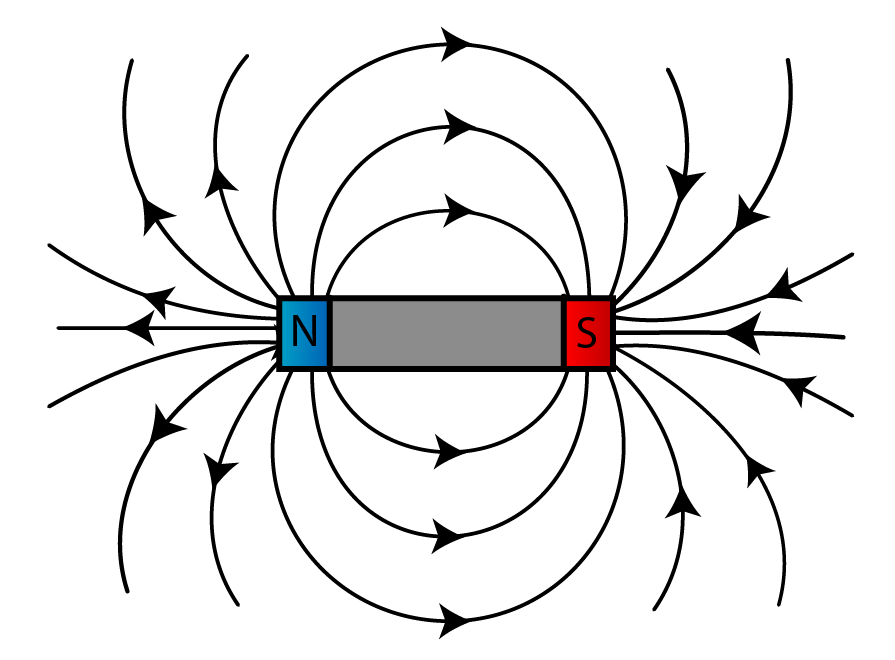
\includegraphics[width=7cm]{img/magnetField.png}
		\end{center}
		\caption{einfaches Magnetfeld}
		\label{fig:einfaches Magnetfeld}
\end{figure}
Die Kraft, welche ein Magnetfeld \( \vec{B}\) auf eine bewegte Ladung mit Ladung \(q\) und Geschwindigkeit \( \vec{v}\) kann mit hilfe von \[
\vec{F_L} = q \vec{v} \times \vec{B}
\]
berechnet werden. Diese Kraft \(F_L\) heisst Lorentzkraft. Die Richtung der Lorentzkraft kann mithilfe der rechten Hand bestimmt werden. Dabei richtet man den Daumen in die Bewegungsrichtung der Positiven Ladung (entgegen der negativen Ladung) und den Zeigefinger in Richtung des Magnetfeldes (von Nord zu Süd). Dann zeigt der Mittelfinger in die Richtung, die die Lorentzkraft auf das bewegte Teilchen ausübt.

Die gesamte elektromagentische Kraft welche auf eine bewegte Ladung ausgeübt wird, kann mithilfe von \[
		\vec{F}_{\textrm{elmag}} = q( \vec{E} + \vec{v} \times \vec{B})
\]


\end{document}
